\documentclass[a4paper, 12pt]{article}

\usepackage[T1]{fontenc}
\usepackage[utf8]{inputenc}
\usepackage[spanish, mexico]{babel}
\usepackage[style=mexican]{csquotes}
\usepackage[margin=2cm,top=2cm,includefoot]{geometry}
\usepackage[spanish, ruled, linesnumbered, lined]{algorithm2e}
\usepackage{amsmath, amsfonts, amssymb, amsthm, amsbsy, cancel}
\usepackage{microtype, parskip}
\usepackage{float, graphicx, subcaption}
\usepackage{circuitikz, tikz, pgfplots}
\usepackage{xcolor}
\usepackage{array, booktabs, multicol, multirow, tabularx}
\usepackage{hyperref, url}
\usepackage{siunitx}
\usepackage{tcolorbox}
\usepackage[style=ieee]{biblatex}
%definir el estilo de lapagina
\usepackage{fancyhdr}
%code
\usepackage{listings}
%Referencias
\addbibresource{code/T4.bib}


%variables de color
\definecolor{greenPortada}{HTML}{69A84F}
\definecolor{CabeceraAcero}{HTML}{5DADE2}
\definecolor{Cabeceraverde}{HTML}{008080}
\definecolor{CabeceraTomate}{HTML}{FF4500}
\definecolor{mymauve}{HTML}{B92FB0}



%cabecera
\setlength{\headheight}{40pt}
\pagestyle{fancy}
\fancyhf{}
\renewcommand{\headrulewidth}{3pt}
\renewcommand{\headrule}{\hbox to \headwidth{\color{CabeceraTomate}\leaders\hrule height \headrulewidth\hfill}}

%variables globales
\newcommand{\lineal}{img/lineal.png}
\newcommand{\nolineal}{img/nol.png}
\newcommand{\ardA}{img/ard_1.png}
\newcommand{\ardB}{img/ard_2.png}
\newcommand{\ardC}{img/ard_3.png}
\newcommand{\boxF}{img/BoxF1_curve.png}
\newcommand{\boxP}{img/BoxP_curve.png}
\newcommand{\dst}{img/create_dst.png}
\newcommand{\pro}{img/label_procss.png}
\newcommand{\yolA}{img/test_yolo.png}
\newcommand{\yolB}{img/test_yolo1.png}
\newcommand{\yolC}{img/test_yolo2.png}
\newcommand{\yolD}{img/yolo_test3.png}
\newcommand{\yolE}{img/yolo_comand.png}

\newcommand{\code}{code/audio.py}


%gestion de hipervinculos
\hypersetup{
    breaklinks=true,
    colorlinks=true,
    citecolor=black,
    filecolor=magenta,
    linkcolor=black, 
    urlcolor=cyan
}

%gestor de codigo
\lstset{
    language=Python,
    basicstyle=\ttfamily\small,
    commentstyle=\color{Cabeceraverde},
    keywordstyle=\color{mymauve},
    numberstyle=\tiny\color{gray},
    stringstyle=\color{CabeceraAcero},
    breaklines=true,
    showstringspaces=false,
    frame=tb,
    numbers=left,
    aboveskip=6mm,
    belowskip=6mm,
    xleftmargin=8mm,
    framexleftmargin=8mm,
    columns=flexible,
    tabsize=4,
    extendedchars=true,
    inputencoding=utf8,
    captionpos=b,
    breakatwhitespace=true,
}

%Encabezado
\title{
    Implementación de un control para sistemas de reproducción utilizando visión artificial con redes neuronales convolucionales
}
\author{		
    Universidad Nacional Autónoma de México\\
    Facultad de Estudios Superiores Cuautitlán\\
    Alonso Vargas Gachuz\\
    Edgar Palomino Alfonso
}
\date{\today}
\cfoot{\thepage}


%inicio de documento
\begin{document} 
    \maketitle  

    \begin{abstract}  
        El uso de las redes neuronales convolucionales \emph{(RNC)} se da a partir de un mejor manejo de imágenes a través de esta, comparado con el uso de redes neuronales con funciones lineales. Esto en conjunto con la capacidad de cómputo dispuesta en aumento, permiten su implementación, ya que a través de una tarjeta gráfica pequeña pero potente se pudo realizar el procesamiento de 4 patrones en diferentes imágenes que se etiquetaron y trataron tomando en cuenta que un conjunto de datos sin un tratamiento adecuado es posible encontrarlo, pero en la realidad no es sencillo realizarlo, lo cual puede dificultar la implementación para un proyecto concreto donde, como este caso, se busca responder a casos específicos como señales de activación para un sistema. de esta manera es como a través de Python, junto a diferentes librerías se logró reconocer la pose de una mano para realizar comandos como play o pausa en un reproductor de música. 
    \end{abstract}  

    \vspace{2ex} 

    \section{Introducción.} 
    El uso de redes neuronales de funciones lineales limitan las dimensiones o parámetros que se pueden trabajar en conjunto para el diseño de estas, ya que en las primeras se busca segmentar la salida a un caso positivo o negativo sobre una línea recta como en la figura~\ref{fig:lin}, cosa que se complica al tener más parámetros de entrada para el análisis como en la figura~\ref{fig:nolin}, este caso se presenta en las imágenes al tener como entradas más de una dimensión para el análisis dejando un sistema más complejo, debido a esto es que se plantean las RNC que además de tener una capa de entrada densa tiene la particularidad de usar redes simples que extraen características particulares, las cuales pasan a otras neurona que agrupa dichas características para determinar un patrón complejo sobre la imagen.\\ 
    Esta propiedad se aplica a la visión por computadora donde tratamos de imitar la manera en que determinamos que algo es una manzana o un perro, si bien existen procesos que ya se encarga de realizar dicho entrenamiento la implementación de un sistema donde podamos hacer play, pausa, subir volumen o bajarlo es lo que se plantea en este proyecto, donde el enfoque que se tiene al mandar estos comandos a un reproductor pudiera manejarse de otra manera, bajo otras circunstancias para que los comando o pose de la mano que se realicen generen una salida distinta sobre un sistema; El motivo de porque hacer uso de esto cuando existen otras opciones bien podría ser porque esto es un comando a distancia donde no se tiene que tocar el dispositivo para interactuar con él, aunque también podemos hacer uso de los comandos por voz, esta propuesta puede fungir como complemento en los ambientes de mucho ruido donde no se factible distinguir la activación de los comandos debido a el ambiente, esta situación se presenta sobre todo si las bocinas y el micrófono se encuentran cerca en el mismo dispositivo, debido a esto se puede hacer uso de estos comandos para crear un sistema más robusto que responda a más tipos de ambientes en la vida cotidiana de los usuarios generado una mayor comodidad en el uso de los dispositivos.\\ 
    Se puede hacer énfasis en que es un comando a distancia donde puede resultar más fácil realizar una seña con la mano para generar una reacción del dispositivo comparando con el tener que gritar para hacer llegar la voz hasta el dispositivo, aunado a esto se debe decir que como todo tiene limitantes ya que requerimos de estar capturando imágenes de manera constante, también se debe ser visibles para la cámara o mejor dicho estar en una posición donde las capturas de la cámara sean aceptables, que no es algo que sea imposible, con esto podemos decir que principalmente brinda una manera distinta de realizar comandos específicos a problemas específicos, solucionando problemas en ambientes de mucho ruido. 

    \begin{figure}[H] 
        \centering 
        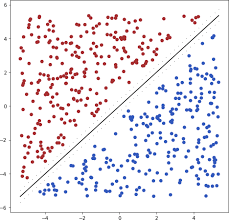
\includegraphics[width=0.35 \linewidth]{\lineal} 
        \caption{Conjunto separable linealmente} 
        \label{fig:lin} 
    \end{figure} 

    \begin{figure}[H] 
        \centering 
        \includegraphics[width=0.35 \linewidth]{\nolineal} 
        \caption{Conjunto no separable de manera lineal} 
        \label{fig:nolin} 
    \end{figure} 

    Cualquier sistema en general agrupa una variedad de elementos los cuales desempeñan diferentes tareas que, en conjunto, son capaces de realizar procesos con gran complejidad. Para cualquier sistema será necesario otorgarle una entrada de la cual se esperará un resultado dependiendo del sistema ya que en algunos casos estas entradas pueden ser objetos o materia que debe ser procesada y en otros se debe manipular información con la cual se espera obtener otro tipo de resultados tal que estos sirvan para regular otros procesos consecuentes, por ejemplo. Para que se pueda recolectar información, el sistema debe contar con sensores de los cuales obtendrá esa comunicación con el entorno que lo rodea de forma que pueda capturar toda la información necesaria para llegar a un resultado satisfactorio, con lo mencionado se puede concluir que cualquier sistema permanece aislado del entorno que lo rodea a menos que se le proporcione un medio para interactuar con su entorno.\\ 
    Los sistemas automatizados hacen uso de sensores con los cuales pueden mantener un control sobre el proceso que llevan a cabo, estos sensores convierten la información del medio físico en señales que pueda interpretar, el problema es que estas son limitadas sumado a que los sistemas no son capaces de inferir sobre los datos para obtener mejores resultados lo que se vuelven inadecuados en determinadas aplicaciones, una de ellas es el reconocimiento de objetos. La forma más utilizada para reconocer elementos del entorno es utilizando sensores de luz con los cuales se pueden llegar a identificar colores entre otros patrones, sin embargo, esto no es suficiente para dotar a un sistema la capacidad de reconocer patrones sobre su entorno. 

    \section{Estado del arte.} 
    La redes convolucionales han tenido una gran auge, ya que pesar de que la teoría de la relación entre el procesamiento de datos de un cerebro biológico y su homologación con el procesamiento de datos por un microprocesador se tenía claro que no existe comparación ya que hay una cantidad mucho mayor de neuronas en un cerebro biológico que microprocesadores en una computadora actual, pero los procesadores cuentan con la capacidad de poseer mayor velocidad ya que como menciona A. Moreno en su tesis el valor de este procesamiento en los humanos es de milisegundo mientras que en la electrónica moderna es de nanosegundos, cosa que brinda una ventaja palpable en el hecho de necesitar poco más de un siglo entre la propuesta de las teorías de estudio del trabajo pionero de Ramón y Cajal en la disertación de la neurona, además de poder hacer énfasis en que fue aún menos tiempo entre las propuestas de Hubel y Wiesel acerca de la corteza visual para tener propuestas y algoritmos que trabajan con el hardware actual para realizar dichas tareas, cosa que puede dejarse ver a través de la historia tomo menos tiempo la evolución de aquellas partes biológicas que estos algoritmos aplicables\cite{artola2019clasificacion}.\\ 
    Si bien esto es palpable debido a este tiempo dimensionado, el artículo de optimización distribuida de redes convolucionales para la clasificación de las imágenes no deja cabida para la duda, ya que su visión de la optimización de RNC distribuidas consta de tener más de una sola computadora dedicada a una sola tarea teniendo un organigrama de principal y secundarios (maestro y esclavos), con el cual logra sacar porcentajes de precisión iguales o mayores a otras arquitecturas propuestas, teniendo en consideración de que el tiempo se reduce al colocar más máquinas dedicadas a la tarea, dejando claro que a mayor cantidad de neuronas el algoritmo puede trabajar de mejor manera, lo cual hace el contraste con todo lo anteriormente dicho\cite{hernandez2019optimizacion}\\ 
    En general lo citado hasta ahora deja de manera clara y básica todo los conceptos necesarios para poder trabajar con RNC, pero el informe de proyecto de grado denominado redes neuronales convolucionales aplicadas a demosaicing y denoising, detalla a profundidad todos los conceptos utilizados, estos nos permite entender de una manera más formal todo aquello se tomará en la sección de conocimientos previos además de proporcionar detalles acerca de cómo es que las imágenes digitales son procesadas para su obtención digital, que aunque como se hace notar en dicho informe todos los fabricantes son libre de llevar a cabo estos procesos tener un panorama general nos permite comprender el procesamiento de imágenes así como los componentes que se procesan y el porqué de los diferentes tratamiento que le daremos a las imágenes una vez estemos implementado la RNC para el reconocimiento patrones sobre diferentes imágenes digitales y que de ser el caso las componentes de color que se requieren para un mejor desempeño de la RNC\cite{balduvin2019redes} 

%conocimientosP 
    \section{Conocimientos previos.} 
    El valor de las RNC está en procesar en paralelo las características de una imagen sin depender de la información que esta proporciona, si bien el orden de dichos valores es importante para el color ya que se utiliza un sistema RGB, el resto de la imagen depende más de las figuras propias del objeto que la RNC pueda identificar para determinar patrones claves que realizan la coincidencia de una imagen con su etiqueta. 

    \subsection{Perceptron.} 
    El perceptrón puede definirse como la función matemática que simula la unidad más básica del pensamiento del ser humano la cual cuenta con entradas, pesos sinápticos, desviaciones y salidas, la cual pondera el valor de cada entrada en función del valor del peso sináptico que se proporciona a dicha entrada, sumada a la desviación de la neurona genera la salida para la decisión final, se puede tener múltiples perceptrones juntos, lo que conforma la redes neuronales densas que como en el nombre se puede percibir es un cúmulo de perceptrones interconectados entre sí para generar un comportamiento en la salida parecido a las decisiones humanas. Dicho comportamiento se define con la función matemática siguiente: 

    \[ 
    f(x) = 
    \begin{cases} 
        0 & \text{si } \sum\limits_{1}^{m} w_i x_i + b < z, 
        \\ 
        1 & \text{en otro caso}. 
    \end{cases} 
    \]

    Donde $m$ es la cantidad de entradas, $xi$ es el valor de la entrada $i$, $b$ corresponde al valor de la desviación asignado a la neurona y $w_i$ corresponde al coeficiente $i$ de la transformación lineal antes mencionada correspondiente al peso sináptico asignado a la entrada $i$. Por último $z$ queda acotado dentro de la función de activación.\\ 
    Debe hacerse notar que es una transformación lineal, lo cual determina que solo podamos hacer uso de dicho perceptrón en conjuntos que sean linealmente separables, en caso contrario las salidas generan errores al no poder hacer una división clara entre los datos. 

    \subsection{Aprendizaje profundo.} 
    El deep learning es un subconjunto de algoritmos pertenecientes al machine learning el cual se diferencia en el tipo de datos que se procesan para su entrenamiento ya que mientras el machine learning utiliza datos estructurados y clasificado para determinar las salidas, el deep learning no requiere dicha estructuración lo que permite trabajar con imágenes de una manera menos compleja ya que no tenemos que estructurara y dar un sentido de cada dato que ingresa si no que el propio algoritmo determina cuales son los datos que importan para procesarlos para de esta manera llegar a la misma salida con la precisión de predicción adecuada sin haber dado la estructuración a cada dato, entiéndase como dato la información de una imagen procesada, esto tiene que ver con la parte de que no se requiere determinar un mapa de bits concreto, si no que a través del proceso se determina cierta cantidad de bits en conjunto dentro de los mapas que son relevantes para determinar dicho objeto.  

    \subsection{Convolución.} 
    La convolución se refiere al proceso matemático de pasar una matriz núcleo que sirve como filtro para extraer datos de un arreglo matricial, es decir es la operación matemática de un arreglo matricial influido por otro, de esta manera podemos pasar los valores del mapa de bits, por un núcleo de mxn valores que altera el valor de todo el arreglo que dicho de esa manera no genera impacto por eso se toma la referencia de filtro, al cambiar el valor de todo el arreglo se puede tomar que se genera otra imagen en base a la imagen original ( se aplica un filtro) afectando los parámetros de dicha imagen, esto ayuda extraer información de los patrones ya que revisamos valores en conjunto y no solo un arreglo de una dimensión en cada iteración, dicho núcleo a través de la convolución del mapa original generará diferentes salidas lo que permite descomponer una imagen compleja en patrones simples, ya que cada uno de los núcleos y cada convolución generará una imagen diferente de salida o mapa de bits distinto de las cuales la red neuronal debe aprender, de esta manera es como se extraen patrones de relevancia para una imagen, también se puede agregar que es el motivo por el que necesitamos data set grades para entrenar una RNC.  

    \subsection{Propagación.} 
    La propagación de los datos se da de una manera típica con un forward, que es decir comienza por la entrada y van hacia la salida ( de adelante hacia atrás), durante este proceso se realizan las operaciones correspondientes como son la convolución, el agrupamiento, se usan las funciones de activación y se determina la salida óptima para el sistema, pero durante la fase de entrenamiento se pueda hacer uso de un algoritmo que mejora los resultados obtenidos a través de la optimización del tiempo empleado que es la propagación hacia atrás o back propagation\\ 
    La propagación hacia atrás es un algoritmo es vital para el entrenamiento de redes neuronales profundas (con más de una capa de neuronas interna), y consiste en propagar el gradiente de la función de costo hacia atrás, actualizando los pesos de cada neurona.\\ 
    La propagación hacia atrás permite ayudar a corregir los pesos actuales de la red, minimizando el error que comete en un conjunto de ejemplos de entrenamiento. Para lograr esto es necesario conocer el gradiente de la función de activación de cada unidad de cada capa. El algoritmo calcula iterativamente para cada capa estos gradientes, tomando como entrada los gradientes calculados para la capa inmediatamente siguiente, esto nos permite tener una “etapa” dedicada a corregir los errores que cada proceso que la red ha cometido, con lo que el siguiente forward tendrá menos errores.\\ 
    Realizando un análisis de este proceso, generamos un entrenamiento con errores gracias a él forward, corregimos los errores en función del peso de la culpa que tiene cada etapa de la red, también se minimiza el error gracias a la propagación hacia atrás, lo cual en el proceso ajusta dichos pesos dejando la lista para que se vuelvan a realizar un forward e iterar de esta manera cada época de la RNC. Haciendo una comparación con los algoritmos genéticos donde escogemos la red que queremos que herede sus genes a la siguiente generación, el algoritmo de back propagation realiza la elección de los pesos que queremos que pases a el siguiente entrenamiento en función de que tanto error han generado o no, si el error es grande la propagación hacia atrás realizará los cambios de los pesos lo que impedirá que dichos errores se lleven a la siguiente época de entrenamiento. 

    \subsection{Capas.} 
    La manera más fácil de comprender todo el proceso que realiza una RNC es haciendo una división por capas, lo que proporciona una abstracción de todos los procesos que se llevan en conjunto y nos permite comprender a gran escala que es lo que se hace por dentro. Partimos de que para cada pixel se requiere tener una neurona dedicada a reconocer que es lo que hay en cada uno de ellos, lo que hace crecer la RNC de una manera acelerada al tener una imagen con mayor cantidad de pixeles o detalles y colores, debido a esto es que se deben de tratar los data set minimizando la cantidad de neuronas que ocuparemos para obtener un resultado aceptable de la tarea, dicho eso podemos organizar el proceso de la tarea e 3 capas.  

    \begin{itemize} 
        \item Entrada: en esta capa es donde se define la cantidad de neuronas que utilizaremos esto depende de la cantidad de pixeles y el canal de color si es que se requiere, una vez estructurada la red pasamos a la siguiente capa.  

        \item Extracción de datos: aquí casi todo el trabajo detallado anteriormente, ya que se genera las convoluciones de las neuronas simples a través de la matrices núcleo, pero como se mencionó se creen diferentes mapas de bits de cada una de las matrices núcleos debido a esto se hace uno de un submuestreo, para agrupar y extraer las características más importantes en de cada filtro, usando generalmente el Max-Pooling.\\ 
        Usando como ejemplo el siguiente caso, podemos suponer que se realiza una Max-Pooling de tamaño 2x2 se recorrerán 32 imágenes de características obtenidas de una imagen de 50x50 píxeles de izquierda a derecha, arriba-abajo, pero en lugar de a un solo píxel, como se toma en las convoluciones, se tomarán de 2x2, es decir 2 de alto por 2 de ancho, solo para preservar el valor más elevado de esos 4 pixeles, de ahí el término Máx. En este caso, usando 2x2 la imagen resultante se reduce a la mitad y quedará una de 25x25 píxeles. Después de este proceso de submuestreo quedan 32 imágenes de 25x25, pasando de haber tenido 80.000 neuronas a 20.000. El descenso es considerable y teóricamente almacenan la información más importante para detectar las características deseadas. de esta manera es como decimos que agrupamos características de neuronas simples a neuronas más complejas ya que extraen y agrupan dichas características para la siguiente convolución, haciendo que cada convolución vea patrones de mayor relevancia, así como con más complejidad.  

        \item Clasificación: esta capa recibe patrones complejos para determinar las probabilidades de que algo sea relevante para el patrón final que determinará la salida o clasificación del objeto, se podría considerar la capa superior que toma la decisión de los porcentajes de la salida según la capa de entrada.  
    \end{itemize} 

    \subsection{Librerías.} 
    Python es el lenguaje de programación más usado para inteligencia artificial, esto debido a que se tiene una inmensidad de librerías y frameworks con lo que se pueden trabajar, en el caso de este proyecto se usará yolo V8 desarrollado por Ultralytics que a grandes rasgos es el modelo de RNC en su versión 8 con el que se entrenó nuestro modelo gracias a su diversificación de fases que consta de clasificar, segmentar, seguir y detectar una pose.\\  
    Al ser un modelo de código abierto se tiene diferentes formas en que se ha mejorado a lo largo del tiempo, pero como se menciona en YOLOv3 An incremental improvement\cite{redmon2018yolov3} cada versión es un puñado de mejoras que lo hacen funcionar de mejor manera, haciendo uso de diferentes técnicas, funciones de activación, procesamiento por lotes, capas de convolución y submuestreo que en conjunto funciona mejoran el desempeño de la RNC, junto a librerías como numpy, pandas, keras y darknet es que funciona.\\  
    En particular Darknet resulta interesante debido a que se basa en yolo pero es una “traducción a C” lo que como bien sabemos es hacer un mejor uso de recurso del hardware al tener mayor control sobre tipos de datos, estructuras de datos, apuntadores y en general mejor manejo de memoria, que para las redes neuronales es valioso, podemos definir que es una optimización de yolo que se implementa al hacer uso de este, tomando como referencia algo similar podemos mencionar a mamba que es la versión en C de Anaconda un manejador de entornos virtuales para Python, con lo que está basado y optimizados para Python pero funciona en C o interactúan con la memoria a través del lenguaje de programación C, esto junto a COCO la cual es un data set enorme que se usó para pre entrenar el modelo hacen de yolo una opción necesaria para avanzar todo el trabajo que hay al querer implementar nuestro proyecto de comandos a través de imágenes.  

    %\clearpage 

%Metodologia 
    \section{Metodología.} 
    El planteamiento que se sigue en este documento se basa en el entrenamiento de la red You Only Look Once (YOLO) para la detección y reconocimiento de señas hechas con las manos a fin de reconocerlas y aplicarlas como comandos para el control de audio en un computador. A continuación se detallan los pasos realizados para entrenar y configurar la red. 

    \subsection{Recolección y tratamiento de los datos.} 
    Las redes convolucionales requieren de una gran cantidad de información, al tener que trabajar con imágenes que poseen varias características es que a la red se le debe proporcionar diferentes datos para entrenamiento, con el fin de mejorar la precisión y confiabilidad en la red. Para este caso se necesita un conjunto particular de datos en los que se tengan determinadas posiciones en las manos, estas servirán para señalizar los controles de medios en el ordenador de las que se eligieron las siguientes propuestas: Mano totalmente abierta o cerrada para la reproducción o pausa, mano abierta con dedo pulgar retraído para aumentar el volumen y mano cerrada con pulgar estirado para reducir el volumen. Para la recolección se realizó un pequeño programa en Python el cual utiliza OpenCV para la captura de imágenes en tiempo real (Figura~\ref{sub:create_dataset}), además de usar Mediapipe(Machine learning) para realizar un seguimiento de las manos, de modo que se pueda obtener una mejor captura y un tratamiento como: ajuste de resolución, medidas y encuadramiento para una mejor detección, se recolectaron en total 160 imágenes por cada señal, haciendo un total de 640 de las cuales se utilizaron 560 para el entrenamiento y 80 para validación. Concluida la tarea de recolección, pasamos al proceso de etiquetado, usando la herramienta labelme, remarcamos el contorno de cada imagen, añadiendo las correspondientes etiquetas(Figura~\ref{sub:label_prcss}). 

    \begin{figure}[H] 
        \centering 

        \begin{subfigure}{0.8\linewidth} 
            \includegraphics[width=\linewidth]{\dst} 
            \caption{Captura de imágenes} 
            \label{sub:create_dataset} 
        \end{subfigure} 

        \begin{subfigure}{0.8\textwidth} 
            \includegraphics[width=\linewidth]{\pro} 
            \caption{Remarcado y etiquetado} 
            \label{sub:label_prcss} 
        \end{subfigure} 

        \caption{Proceso de creación del set de datos} 
    \end{figure} 

    Al remarcar y etiquetar las imágenes, la herramienta labelme generará un archivo tipo JSON, dónde se encuentran las etiquetas y los puntos generados previamente, además de incluir algunos otros datos, sin embargo, la red YOLO únicamente acepta el formato .txt donde se indiquen los puntos remarcados en el proceso de etiquetado. Para hacer la conversión se utilizó la herramienta labelme2yolo la cual realiza esta tarea de forma automática. Al usar la herramienta nos arrojará una carpeta con dos carpetas dentro y un archivo de tipo yaml. Las carpetas generadas contienen las imágenes del set de datos y las etiquetas generadas con extensión .txt, el archivo yaml es requerido por la red, tiene el objetivo de indicarle donde encontrar los archivos de entrenamiento y validación respectivamente. 

    \subsection{Entrenamiento de la red neuronal.} 
    Con el set de datos completo, podemos proceder al entrenamiento de la red neuronal YOLO, para comenzar es necesario conseguir la librería Ultralytics de Python, dónde obtendremos la herramienta para el entrenamiento, opcionalmente se puede instalar PyTorch con la cual es posible trabajar utilizando la tarjeta gráfica del computador, acelerando el proceso de entrenamiento, aunque se puede optar por usar la CPU en este caso se optó por incluirlo. Para comenzar el entrenamiento utilizamos el comando yolo, indicándole los parámetros deseados para comenzar el entrenamiento(figura~\ref{fig:yolo_train}). 

    \begin{figure}[H] 
        \centering 
        \includegraphics[width=0.98 \linewidth]{\yolE} 
        \caption{Proceso de entrenamiento de la red YOLO, en los parámetros se indican de izquierda a derecha: tarea de segmentación, modo de entrenamiento, 60 épocas, ruta del set de datos, versión requerida, resolución de las imágenes y cantidad de imágenes para la tarea} 
        \label{fig:yolo_train} 
    \end{figure} 

    Este proceso arrojará una carpeta donde se tendrán los resultados del entrenamiento, mostrando la matriz de confusión, las gráficas de precisión, una carpeta con los archivos de pesos obtenidos del entrenamiento, algunas de las imágenes para la validación entre otras cosas útiles para el análisis de los resultados. Lo más importante dentro de la carpeta son los archivos que contienen los pesos cuya extensión es .pt, existen dos archivos los cuales son best y last, siendo el archivo best quien contiene los pesos que entregan mejores resultados.  

    \subsection{Control de medios.} 
    Existe una gran cantidad de librerías que proporciona la comunidad de Python, entre estas existen algunas que nos brindan control sobre las funcionalidades del sistema operativo y sobre los medios. Como primera instancia se realizó un programa para el control del audio maestro en el ordenador utilizando la librería pycaw, la cual otorga algunos métodos sobre el control de audio. Otra librería importante es pyautogui la cual permite simular algunas opciones de teclas usadas en el sistema operativo, usándola podemos simular el control del botón play/pause, uno de los comandos por defecto de teclado que nos entregará el control de reproducción sobre cualquier aplicación que reproduzca audio en el ordenador. 

    %\clearpage 

    \lstinputlisting[language=Python]{\code} 
    En resumen, el código obtiene el parámetro requerido que puede ser cualquiera de las 4 opciones (reproducción, pausa, subir o bajar volumen), en función de dicha entrada realizará una de dichas acciones, la entrada es resultante del proceso de predicción de la red neuronal entrenada. 

    \subsection{Pruebas de funcionamiento.} 
    Al conseguir los pesos para la red neuronal, es posible exportarlos para realizar pruebas, la librería Ultralytics permite instanciar el modelo en un objeto, este solo requiere de dichos pesos para poder funcionar de acuerdo al entrenamiento realizado. Para hacer las pruebas nuevamente se realizó un seguimiento de la mano para obtener mejores entradas y que se adecuaran con los datos de entrenamiento, estas fueron pasadas al modelo y con ayuda de las funciones del mismo, se obtuvieron las predicciones al mostrarlas en la pantalla junto con el seguimiento de la mano. 

    \begin{figure}[H] 
        \centering 

        \begin{subfigure}{0.45\linewidth} 
            \includegraphics[width=\linewidth]{\yolA} 
            \caption{Prueba para play} 
            \label{sub:play} 
        \end{subfigure} 

        \begin{subfigure}{0.45\linewidth} 
            \includegraphics[width=\linewidth]{\yolB} 
            \caption{Prueba para pause} 
            \label{sub:pause} 
        \end{subfigure} 

        \begin{subfigure}{0.45\linewidth} 
            \includegraphics[width=\linewidth]{\yolC} 
            \caption{Prueba para V-} 
            \label{sub:v+} 
        \end{subfigure} 

        \begin{subfigure}{0.45\linewidth} 
            \includegraphics[width=\linewidth]{\yolD} 
            \caption{Prueba para V+} 
            \label{sub:v-} 
        \end{subfigure} 

        \caption{Resultados de las predicciones del modelo entrenado} 
    \end{figure} 

    \subsection{Implementación de resultados.} 
    Comprobado el funcionamiento, se procedió a implementar la red de modo que controlara los medios del ordenador, para verificar el funcionamiento más adecuadamente, se empleó una pantalla LCD en la cual se despliegan las opciones detectadas por la red, de modo que, cuando se detecta una opción, un microcontrolador desplegará en un LCD la conclusión obtenida. 

    \begin{figure}[H]
        \centering 

        \begin{subfigure}[h]{0.6\linewidth} 
            \includegraphics[width=\linewidth]{\ardA} 
            \caption{Acción de reproducción/pausa} 
        \end{subfigure} 

        \begin{subfigure}[h]{0.6\linewidth} 
            \includegraphics[width=\linewidth]{\ardB} 
            \caption{Reducción del volumen} 
        \end{subfigure} 

        \begin{subfigure}[h]{0.6\linewidth} 
            \includegraphics[width=\linewidth]{\ardC} 
            \caption{Aumento de volumen} 
        \end{subfigure} 

        \caption{Pruebas con el LCD} 
    \end{figure} 

    \clearpage 

    \section{Análisis de resultados.} 
    La herramienta para el entrenamiento proporciona en su salida una serie de archivos con los resultados del entrenamiento, dichos elementos hacen más fácil el análisis detallado sobre el desempeño de la red neuronal.\\ 
    Primero hay que analizar las curvas de confianza. 

    \begin{figure}[H] 
        \centering 

        \begin{subfigure}{0.75\linewidth} 
            \includegraphics[width=\linewidth]{\boxF} 
            \label{F1_curve} 
            \caption{Exactitud del modelo} 
        \end{subfigure} 

        \begin{subfigure}{0.75\linewidth} 
            \includegraphics[width=\linewidth]{\boxP} 
            \label{P_curve} 
            \caption{Precisión del modelo} 
        \end{subfigure} 

        \caption{Curvas de confianza} 
    \end{figure} 

    Con estas gráficas es posible visualizar que la exactitud del modelo aumenta cuando el valor de confianza es bajo en la mayoría de los casos y que la precisión aumenta cuando la confianza del modelo es mayor, sobre la gráfica de exactitud podemos concluir en que ciertos traslapes en la identificación de las formas, lo cual es entendible pues de cierta forma son muy parecidas las formas que debe identificar como cuando la mano está totalmente abierta y cuando la mano está abierta pero con el pulgar enroscado, por lo que existirá cierto traslape en algunas de las posiciones donde habrá error, para mejorar el reconocimiento se debería optar por añadir más imágenes para el entrenamiento, ya que 140 son bastante pocas. 

    \section{Conclusiones.} 
    La implementación de soluciones a problemas es complejo debido a que necesitas más de un área de conocimiento para poder llevar a cabo dicha acción, este trabajo nos demostró esta parte ya que desde el momento en que se planteó el proyecto surgió el primer obstáculo que fue conseguir un data set grande con las imágenes que se requieren, cosa que no fue posible encontrar, esto nos llevó a profundizar en data set, métodos para tratar imágenes todo para obtener un data set en forma. Así como ese detalle fueron surgiendo más problemáticas pero Python tiene una solución casi para todo, con lo que se pudo surfear estos inconvenientes, sobra decir que entender cómo funcionan cada una de las librerías fue otra gran tarea, que nos permite la conclusión de que lo esencial de Python ayuda en cualquier lenguaje o que lo esencial de cualquier lenguaje ayuda a comprender dichas librerías, también tenemos el hecho de que el trabajo open source y la tecnología en general carece de un núcleo común en cuanto a el desarrollo, los estándares que se define para cada tecnologías son diferentes, esto puede hacer que pierdas un poco el sentido del porqué de esas cosas, pero debe destacarse que los problemas que se resuelven son diferentes, así como las maneras en que una persona implementará una solución, lo que me lleva a decir que la ingeniería puede pecar de “ingenio”, muchas soluciones a un mismo problema de diferentes maneras, pero esto tiene el inconveniente de no poseer el tiempo que este requiere, ya que en el camino se bifurca las ideas terminando en procesos distintos y con cientos de soluciones al punto de que analizar dichas opciones es absurdo ya que esto sería más desgastante que resolver el problema en sí.\\ 
    Contribuir a dar una nueva solución que termina convirtiéndose en un problema es otro tema que se puede tratar, porque se requiere siempre escalar los modelos, crear sistemas robustos que al hacer la unión de un sistema A con un sistema B generalmente rompe alguno de los dos, junto a la idea de jugar con el hardware y software para obtener un producto pulido, cada proyecto es un mundo lo que nos permite concluir que el trabajo en equipo, lo ciclos de trabajo, las herramientas que se construyen cobran sentido al enfrentarse a todos estos escenarios que no paran de ser tan diversos, durante la carrera se acotan todos los problemas para su entendimiento pero en un proyecto tangible las soluciones se desfragmenta, con lo que se termina haciendo la observación de que resolver problemas es algo que no es cierto del todo, solo se dan un puñado de nuevas característica que hace un mejor desempeño sobre una tarea.  

    \clearpage

    \printbibliography 

\end{document} 


